\section{Extra Challenge 3}
Σε αυτή την ενότητα θα παρουσιαστούν οι διάφορες ενέργειες που πραγματοποιήθηκαν εκτός από τα challenges που αναλύθηκαν προηγουμένως.

\subsection{Περιβάλλον chroot για καλύτερο performance}\label{seq:chroot}
Καθώς η προσομοίωση σε virtual machine εισάγει σημαντικές καθυστερήσεις έγινε τοπική εγκατάσταση σε περιβάλλον \href{https://en.wikipedia.org/wiki/Chroot}{chroot}.
Αυτή η μέθοδος δουλεύει και σε μη debian-based Linux συστήματα.
Απαραίτητα προγράμματα αποτελούν τα \href{https://linux.die.net/man/8/debootstrap}{\texttt{debootstrap}}
και \href{https://linux.die.net/man/1/schroot}{\texttt{schroot}}.

Το βασικό configuration παρουσιάζεται στη~\ref{code:schroot-config}.
\begin{code}
\caption{schroot config file}\label{code:schroot-config}
\begin{minted}{ini}
[indigo_trusty]
description=Ubuntu 14.04 for installing ROS Indigo
directory=/srv/chroot/indigo_trusty
root-groups=root
type=directory
users=orestis
personality=linux
preserve-environment=false
aliases=default
\end{minted}
\end{code}

Στη συνέχεια καταγράφονται οι βασικές εντολές που χρησιμοποιήθηκαν για την εγκατάσταση του συστήματος.
\begin{code}
\caption{Εγκατάσταση βασικού συστήματος}
\begin{minted}{bash}
# Εγκατάσταση ubuntu 14.04 μέσω bootstrap:
sudo mkdir -p /srv/chroot/indigo_trusty
sudo debootstrap --variant=buildd --arch=amd64 trusty /srv/chroot/indigo_trusty http://archive.ubuntu.com/ubuntu/
\end{minted}
\end{code}
\begin{code}
\caption{Απαραίτητα mount, εντολές ως root}
\begin{minted}{bash}
# Από https://wiki.archlinux.org/index.php/change_root:
cd /srv/chroot/indigo_trusty/
mount -t proc proc proc/
mount --rbind /sys sys/
mount --rbind /dev dev/
mount --rbind /run run/
cp /etc/resolv.conf /srv/chroot/indigo_trusty/etc/resolv.conf
cp /etc/hosts /srv/chroot/indigo_trusty/etc/hosts
\end{minted}
\end{code}
\begin{code}
\caption{Εγκατάσταση ros και προγραμμάτων}
\begin{minted}{bash}
sudo schroot -c indigo_trusty  # Αλλαγή περιβάλλοντος.
# Μέσα στο chroot
apt-key update
apt-get install sudo vim git bash wget -y  # Βασικά, χρήσιμα προγράμματα.
locale-gen en_US en_US.UTF-8
dpkg-reconfigure locales
\end{minted}
\end{code}
\begin{code}
\caption{Εγκατάσταση απαραίτητων πακέτων ros}
\begin{minted}{bash}
schroot -c indigo_trusty  # Αλλαγή περιβάλλοντος ως απλός χρήστης.
sudo sh -c 'echo "deb http://archive.ubuntu.com/ubuntu trusty universe" >> /etc/apt/sources.list'
sudo sh -c 'echo "deb http://packages.ros.org/ros-shadow-fixed/ubuntu trusty main" > /etc/apt/sources.list.d/ros-latest.list'
wget http://packages.ros.org/ros.key -O - | sudo apt-key add -
sudo apt-key update
sudo apt-get update
sudo apt-get install python-rosdep
sudo rosdep init
rosdep update
sudo apt-get install git mercurial ros-indigo-map-server python-pip libffi-dev -y
sudo apt-get install gfortran libopenblas-dev liblapack-dev
sudo dpkg-reconfigure -phigh -a  # Αν χρειαστεί

mkdir -p ~/catkin_ws/src
cd ~/catkin_ws/src
catkin_init_workspace
git clone https://github.com/stdr-simulator-ros-pkg/stdr_simulator.git
cd stdr_simulator
git checkout autonomous_systems
cd ~/catkin_ws/src/
git clone https://github.com/etsardou/intelligent_robot_systems_2016.git
cd ~/catkin_ws
source /opt/ros/indigo/setup.bash --extend

# Υπόλοιπα απαραίτητα για το project
rosdep install --from-path src --rosdistro indigo -i -y
sudo pip install cython
sudo pip install cffi scikit-image
sudo easy_install scipy
\end{minted}
\end{code}
\begin{code}
\caption{Build}
\begin{minted}{bash}
cd ~/catkin_ws
catkin_make -j1
cd ./src/intelligent_robot_systems_2016/art_autonomous_exploration/src
make
\end{minted}
\end{code}

\subsection{Βίντεο Εξερεύνησης}
\begin{itemize}
    \item Το video της εξερεύνησης σε κανονική ταχύτητα:
          \url{https://vimeo.com/217997108}.
    \item Το video της εξερεύνησης σε επιτάχυνση:
          \url{https://vimeo.com/218002955}.
\end{itemize}
Τα βίντεο δείχνουν το παράθυρο του RViz και παράλληλα το output στο terminal.
Η βιντεοσκόπηση έγινε σε περιβάλλον \hyperref[seq:chroot]{chroot}.

\subsection{Δημιουργία προβληματικών μονοπατιών}\label{section:uniform-sampling}
\begin{figure}[htb]
    \centering
    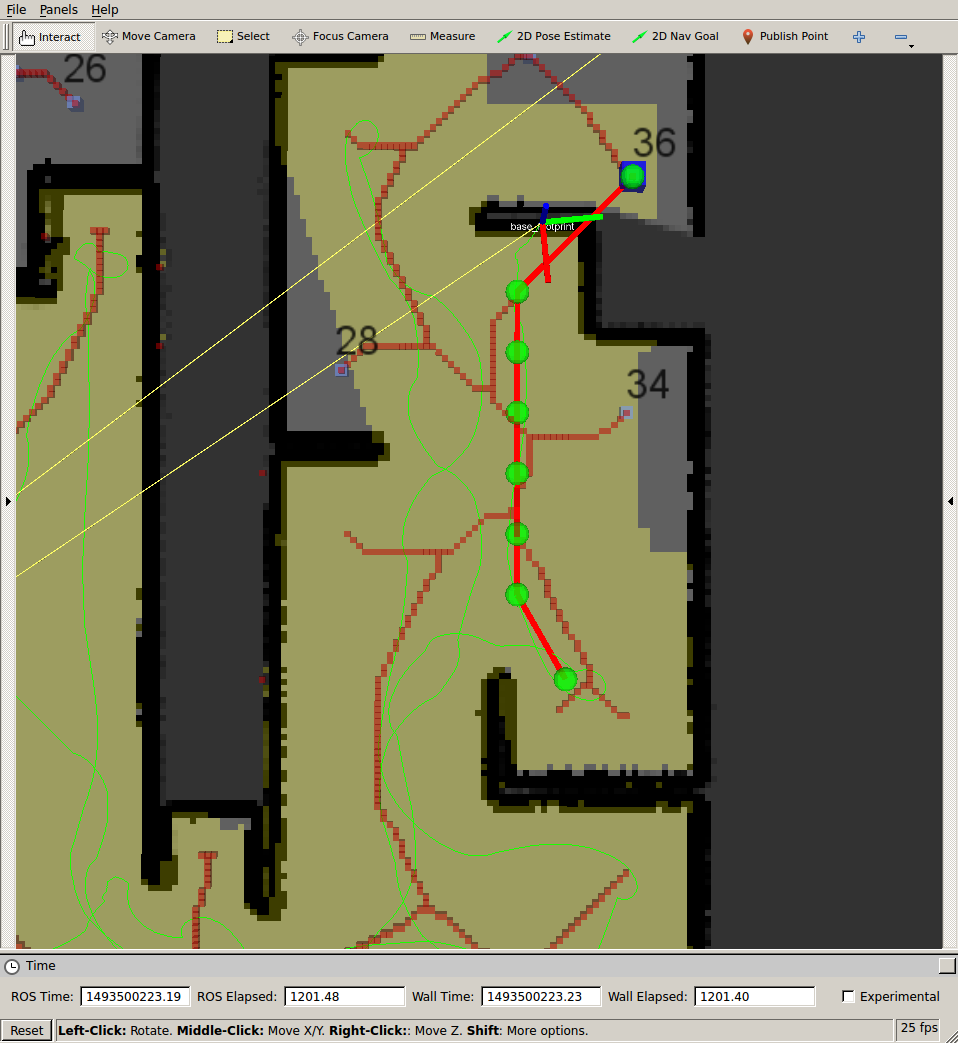
\includegraphics[width=0.49\linewidth, keepaspectratio]{screens/path-problem-1}
    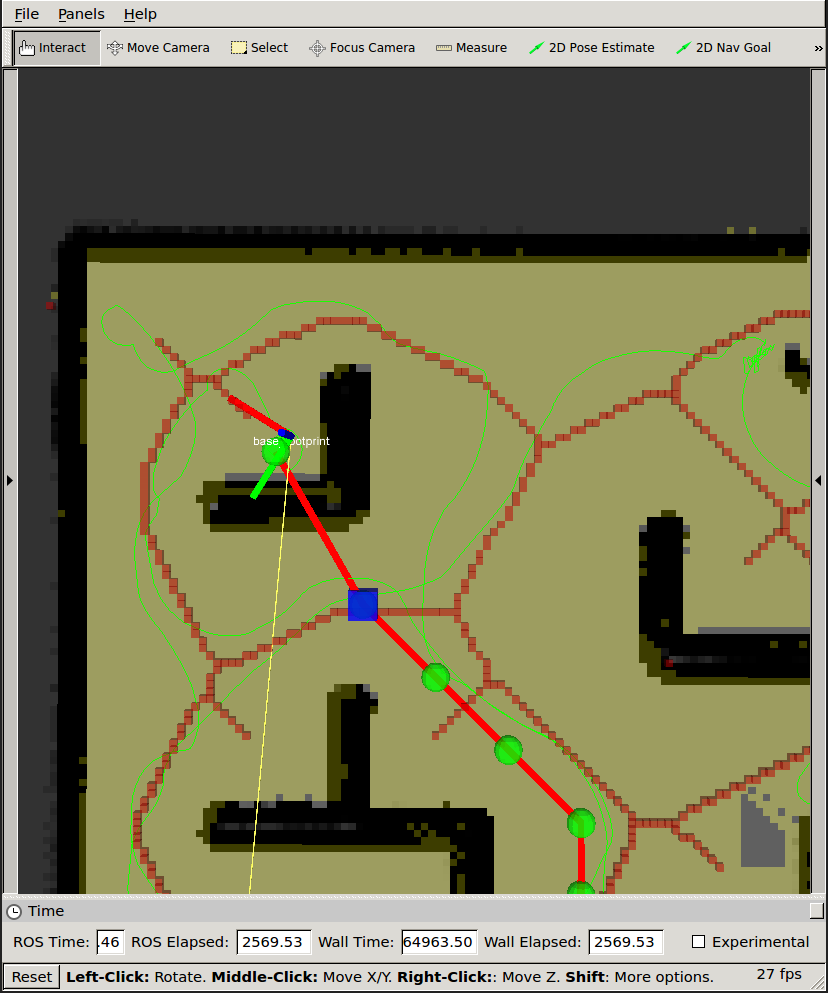
\includegraphics[width=0.49\linewidth, keepaspectratio]{screens/path-problem-2}
    \caption{Προβληματική δημιουργία μονοπατιών}\label{fig:path-problem}
\end{figure}

Ένα βασικό πρόβλημα που αντιμετωπίστηκε είναι η δημιουργία μονοπατιών που περνάν μέσα από εμπόδια όπως φαίνεται στο σχήμα~\ref{fig:path-problem}.
Για τη βελτίωση έγιναν οι εξής αλλαγές:
\begin{enumerate}
    \item Μεταβολή της παραμέτρου \texttt{uniform\_sampling\_step} από \texttt{0.5} σε \texttt{0.3}
          και της \texttt{uniform\_minimum\_distance\_from\_walls} από \texttt{0.0} σε \texttt{0.3}
          στο αρχείο \path{./art_ogmpp/ogmpp_planners/cfg/prms_parameters.yaml}.
          Αυτό λύνει οριστικά το πρόβλημα αλλά καθιστά το path planning πολύ αργό.

    \item Προσπάθεια διαγραφής γειτόνων που περνάνε μέσα από εμπόδια στο αρχείο
          \path{./art_ogmpp/ogmpp_planners/src/ogmpp_planners/ogmpp_prms/ogmpp_uniform_sampling.cpp}
          Το πρόβλημα δε λύθηκε αποκλειστικά με αυτή τη προσέγγιση.
          Το σύνολο των αλλαγών που πραγματοποιήθηκαν μπορούν να βρεθούν με την εντολή:\\
          \mintinline{bash}!git diff 549b260^1 549b260!.
\end{enumerate}
